% =========================================================
% CHAPTER 4
% =========================================================

\chapter{Kiến trúc và thiết kế hệ thống}
\label{Chapter4}

% =========================================================
\section{Kiến trúc tổng thể hệ thống}
% =========================================================

Từ các yêu cầu đã phân tích ở Chương~\ref{Chapter3}, hệ thống được thiết kế theo mô hình nhiều thành phần, gồm giao diện người dùng, backend API, cơ sở dữ liệu và agent-worker. Kiến trúc hỗ trợ toàn bộ vòng đời kiểm thử: quản lý project, sinh và lựa chọn test case, tạo automation test script bằng agent, lưu replay script, thực hiện kiểm thử hồi quy và phân tích kết quả.

Các mục tiêu thiết kế chính gồm:

\begin{itemize}
    \item \textbf{Tách biệt trách nhiệm}: frontend xử lý tương tác; backend quản lý nghiệp vụ và dữ liệu; agent-worker thực thi kiểm thử trên trình duyệt.
    
    \item \textbf{Hỗ trợ ngôn ngữ tự nhiên}: tester có thể mô tả yêu cầu hoặc mục tiêu kiểm thử bằng prompt.
    
    \item \textbf{Kiểm soát kết quả do AI sinh}: tester xem xét và lựa chọn test case trước khi sử dụng để tạo automation test script.
    
    \item \textbf{Kết hợp agent và replay script}: agent hỗ trợ tạo script ban đầu; replay script được ưu tiên trong kiểm thử hồi quy.
    
    \item \textbf{Lưu vết thực thi}: mỗi test run lưu trạng thái, verdict, step log, screenshot, evidence và thông tin lỗi.
    
    \item \textbf{Hỗ trợ bảo trì}: Object Repository, assertion và locator fallback hỗ trợ xử lý khi giao diện website thay đổi.
    
    \item \textbf{Kiểm soát chi phí và tài nguyên}: giảm số lần gọi LLM khi đã có replay script và giới hạn số phiên trình duyệt chạy đồng thời.
\end{itemize}

% ---------------------------------------------------------
\subsection{Kiến trúc component cấp hệ thống}

Kiến trúc tổng thể gồm frontend, backend API, cơ sở dữ liệu, agent-worker, mô hình ngôn ngữ lớn, thành phần tự động hóa trình duyệt và website mục tiêu. Các thành phần giao tiếp thông qua HTTP API và callback.

\begin{figure}[H]
    \centering
    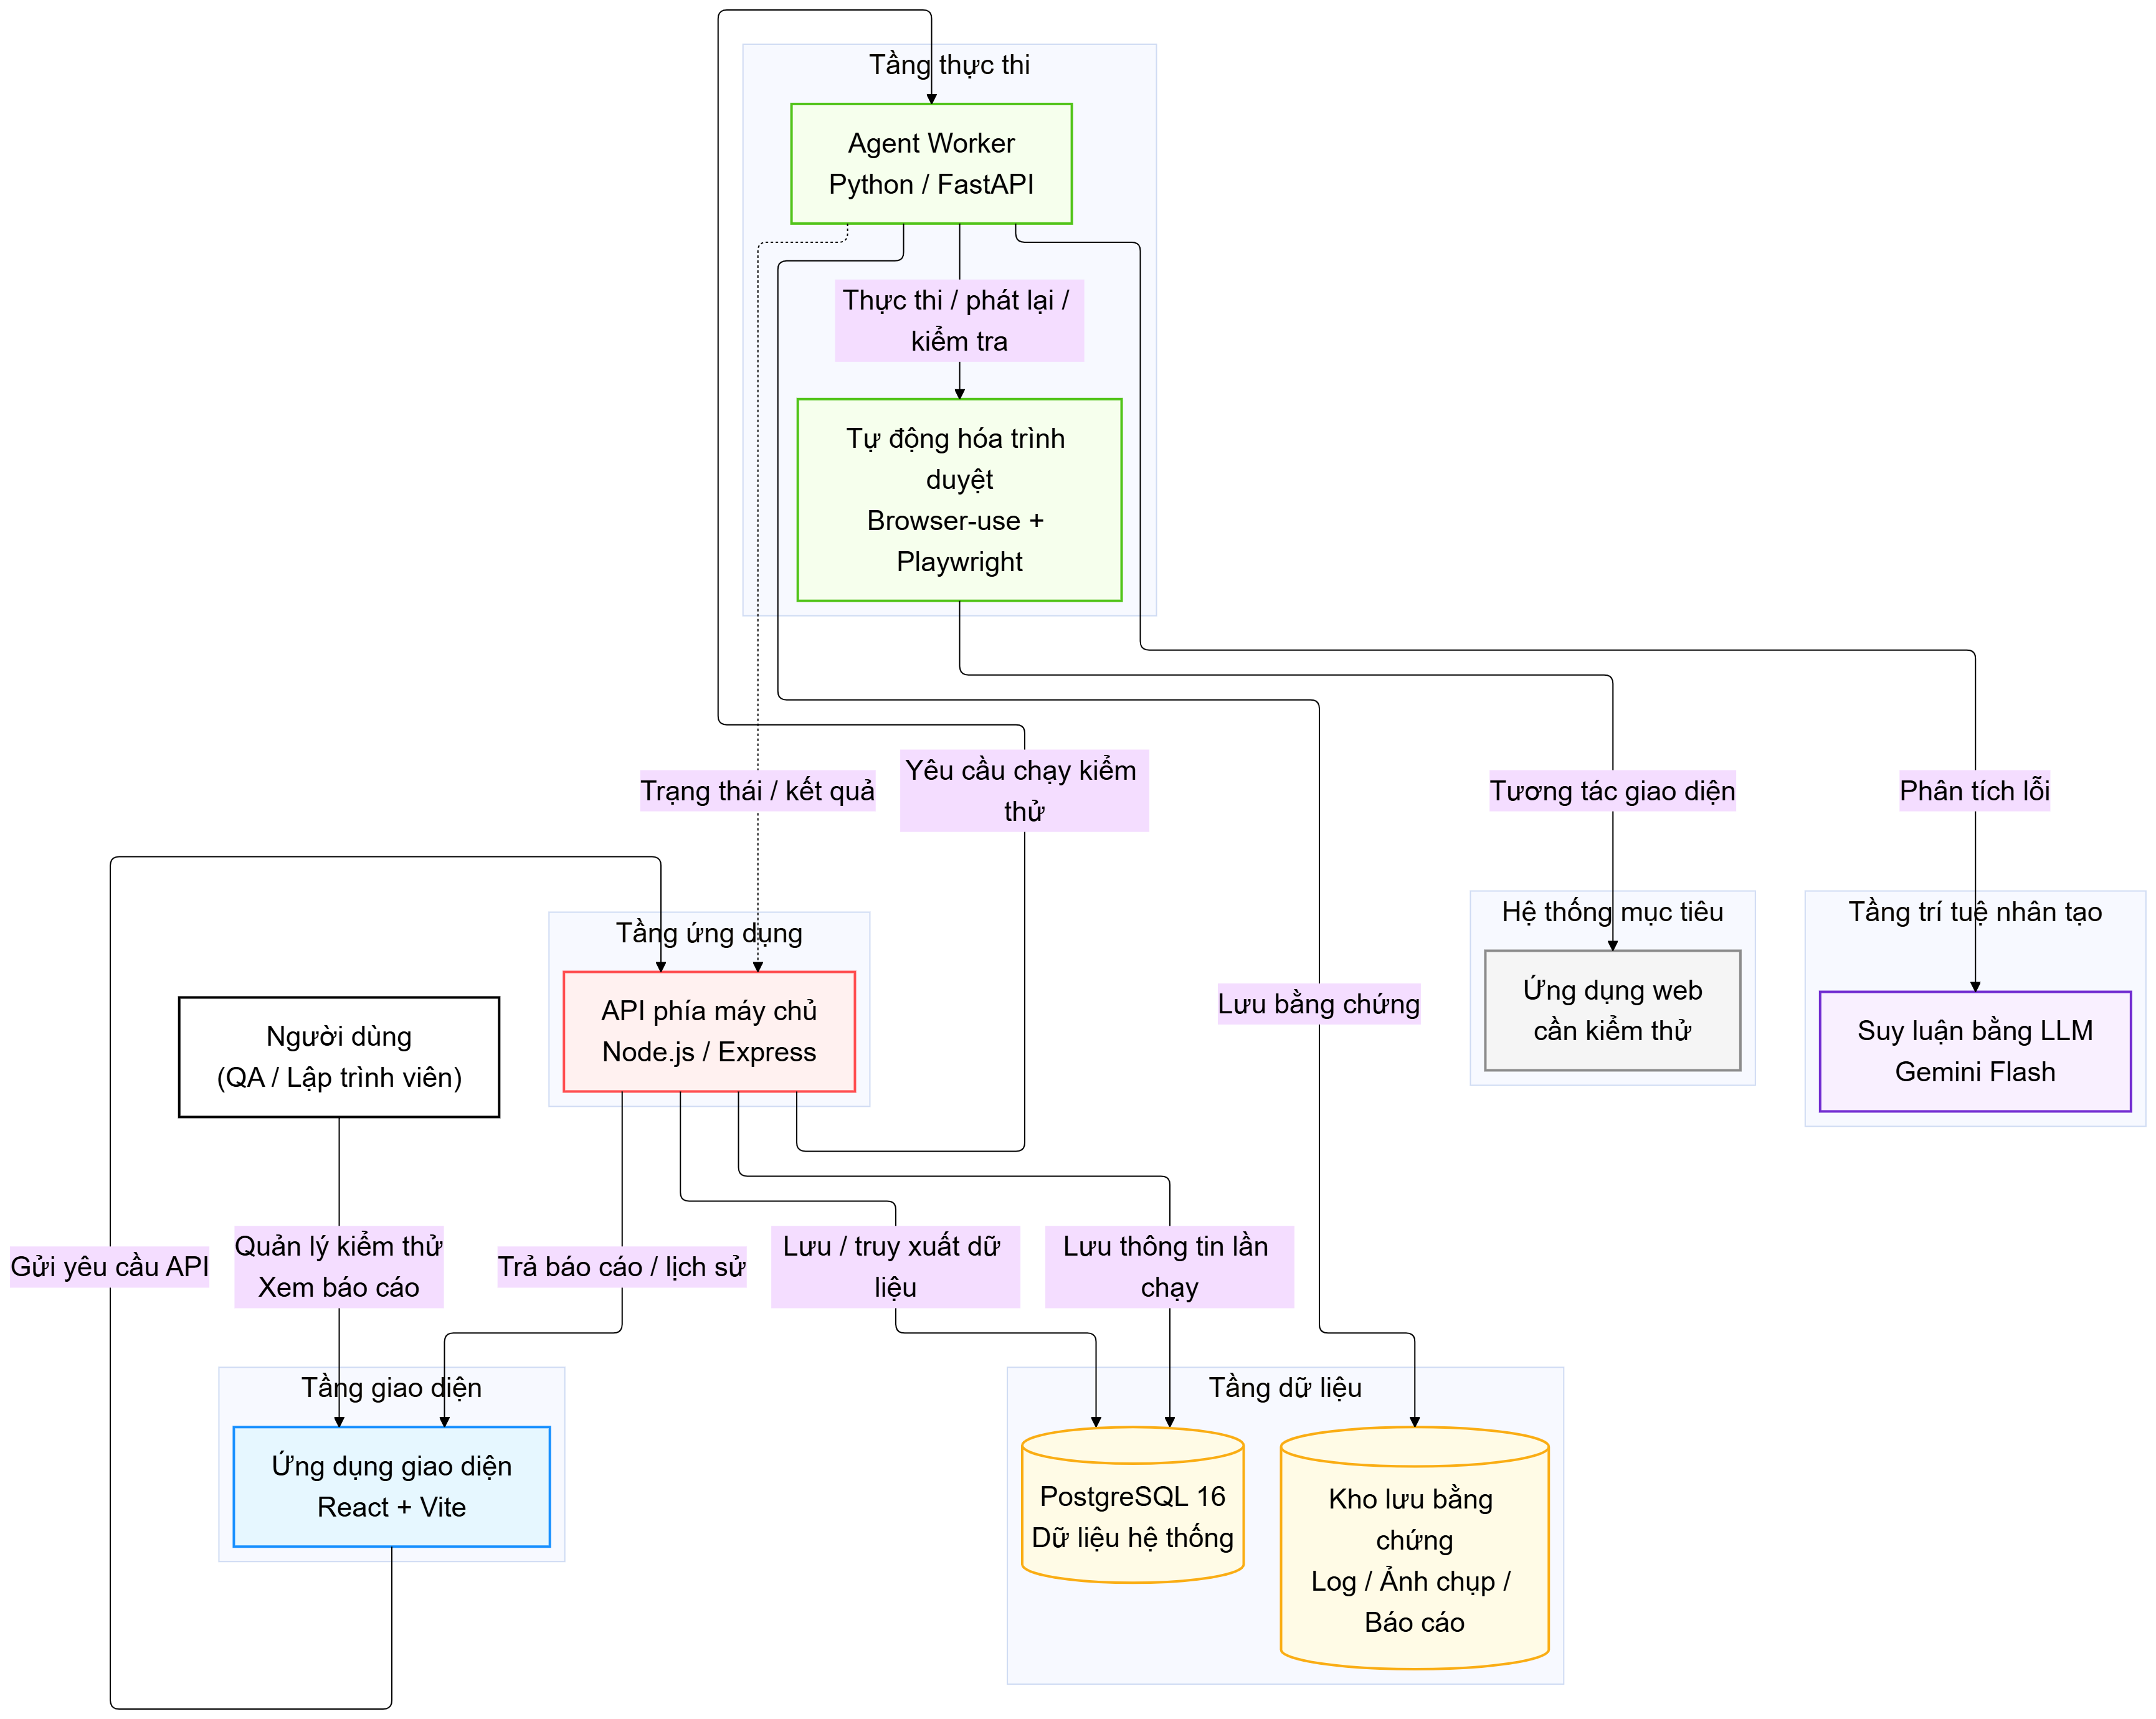
\includegraphics[
        width=\textwidth,
        height=0.78\textheight,
        keepaspectratio
    ]{images/chapter4/system_architecture.png}
    \caption{Kiến trúc tổng thể của hệ thống kiểm thử tự động website}
    \label{fig:system_architecture}
\end{figure}

Tester thao tác trên frontend để quản lý project, sinh và lựa chọn test case, quản lý dữ liệu kiểm thử và theo dõi kết quả. Backend kiểm tra quyền truy cập, xử lý nghiệp vụ, lưu dữ liệu và gửi yêu cầu thực thi sang agent-worker.

Agent-worker phối hợp với LLM và thành phần tự động hóa trình duyệt để tạo automation test script hoặc chạy replay script. Kết quả thực thi được gửi về backend thông qua callback để lưu trữ và hiển thị trên frontend.

% ---------------------------------------------------------
\subsection{Định hướng công nghệ}

Bảng~\ref{tab:chapter4_technology_components} trình bày định hướng công nghệ theo từng thành phần. Các thư viện, phiên bản và chi tiết tích hợp được trình bày tại Chương~\ref{Chapter5}.

\begin{table}[H]
\centering
\caption{Định hướng công nghệ theo thành phần}
\label{tab:chapter4_technology_components}
\renewcommand{\arraystretch}{1.2}
\begin{tabular}{|p{4.0cm}|p{4.2cm}|p{6.0cm}|}
\hline
\textbf{Thành phần} &
\textbf{Loại công nghệ} &
\textbf{Vai trò} \\
\hline

Giao diện người dùng &
Frontend web framework &
Cung cấp giao diện xác thực, quản lý project, sinh và lựa chọn test case, quản lý cây thư mục Test Cases, dataset, test suite, Object Repository và report. \\
\hline

Backend API &
Web API framework &
Xử lý nghiệp vụ, quản lý dữ liệu, xác thực tester và điều phối yêu cầu thực thi. \\
\hline

Cơ sở dữ liệu &
Hệ quản trị cơ sở dữ liệu quan hệ &
Lưu project, lịch sử sinh test case, test case ứng viên, test case chính thức, replay script, test run, evidence, dataset và dữ liệu hỗ trợ. \\
\hline

Agent-worker &
Worker service &
Khởi tạo trình duyệt, chạy agent hoặc replay script và trả kết quả về backend. \\
\hline

Tự động hóa trình duyệt &
Browser automation framework &
Điều khiển trình duyệt, thực hiện action, assertion và ghi nhận screenshot. \\
\hline

AI/LLM &
Mô hình ngôn ngữ lớn &
Hỗ trợ sinh test case, sinh dữ liệu, suy luận hành động và phân tích kết quả thực thi. \\
\hline
\end{tabular}
\end{table}

% =========================================================
\section{Thiết kế các thành phần hệ thống}
% =========================================================

\subsection{Thiết kế giao diện người dùng}

Giao diện được thiết kế theo vòng đời kiểm thử: xác thực tester, quản lý project, sinh và lựa chọn test case, tạo automation test script, tổ chức test case, chuẩn bị dữ liệu kiểm thử, chạy kiểm thử hồi quy và xem kết quả.

Các màn hình chính gồm đăng nhập, đăng ký, Dashboard, Generate Testcase, Test Cases, Test Case Detail, Test Suite Detail, Data, Objects và Test Runs.

Trang \textit{Generate Testcase} là khu vực để tester nhập yêu cầu bằng ngôn ngữ tự nhiên, sinh danh sách test case đề xuất và lựa chọn các test case phù hợp. Giao diện có thể được chia thành nhiều section để tester xử lý các nhóm yêu cầu khác nhau. Các section chỉ đóng vai trò tổ chức không gian làm việc và không được xem là một chức năng nghiệp vụ độc lập.

Các test case được lựa chọn tiếp tục được sử dụng làm đầu vào cho agent để tạo automation test script. Sau khi script được tạo và xác nhận, test case cùng replay script được chuyển sang trang \textit{Test Cases}.

Trang \textit{Test Cases} đóng vai trò là kho lưu trữ các test case chính thức. Test case được tổ chức theo cấu trúc cây thư mục để tester phân nhóm theo chức năng, module hoặc luồng nghiệp vụ.

Thiết kế ưu tiên việc tester không phải viết script ngay từ đầu. Các chức năng nhập yêu cầu, lựa chọn test case, tạo script bằng agent, chạy replay script, chọn dataset và xem evidence được tổ chức theo một luồng thao tác thống nhất.

% ---------------------------------------------------------
\subsection{Thiết kế backend API}

Backend API được tổ chức theo các nhóm tài nguyên như authentication, projects, test case generations, test cases, datasets, test suites, test runs, execution scripts, evidences và reports.

Backend chịu trách nhiệm:

\begin{itemize}
    \item Xử lý đăng ký, đăng nhập, Google OAuth và khôi phục mật khẩu.
    
    \item Kiểm tra quyền truy cập theo tester và project.
    
    \item Quản lý lịch sử sinh test case và các test case ứng viên.
    
    \item Lưu lựa chọn của tester và quản lý test case chính thức.
    
    \item Tạo test run và gửi yêu cầu thực thi sang agent-worker.
    
    \item Nhận callback step, evidence và kết quả cuối cùng.
    
    \item Lưu replay script và liên kết script với test case tương ứng.
\end{itemize}

Backend không trực tiếp điều khiển trình duyệt mà chỉ điều phối các yêu cầu thực thi sang agent-worker.

% ---------------------------------------------------------
\subsection{Luồng giao tiếp tổng quan}

Frontend gửi yêu cầu nghiệp vụ đến backend. Backend kiểm tra dữ liệu, quyền truy cập và lưu các bản ghi cần thiết.

Đối với yêu cầu sinh test case, backend gọi LLM và trả danh sách test case đề xuất về frontend. Sau khi tester lựa chọn test case và yêu cầu tạo script, backend tạo test run và gửi yêu cầu sang agent-worker.

Agent-worker chạy test trên trình duyệt, ghi nhận step log, screenshot, action history và evidence, sau đó callback kết quả về backend. Khi phiên chạy thành công, action history được chuẩn hóa thành replay script để tester xem xét và xác nhận.

% =========================================================
\section{Thiết kế dữ liệu và lưu trữ}
% =========================================================

Cơ sở dữ liệu được thiết kế xoay quanh vòng đời kiểm thử, từ tạo project, sinh test case đề xuất, lựa chọn test case, tạo automation test script đến chạy kiểm thử hồi quy, lưu evidence và phân tích kết quả.

Chương này chỉ trình bày các bảng cốt lõi và nhóm dữ liệu hỗ trợ. Toàn bộ schema vật lý, migration, chỉ mục và ràng buộc chi tiết không thuộc phạm vi trình bày chính.

Các nguyên tắc thiết kế dữ liệu gồm:

\begin{itemize}
    \item \textbf{Truy vết đầy đủ}: mỗi test run phải liên kết được với project, test case, replay script, dataset và evidence liên quan.
    
    \item \textbf{Tách test case đề xuất và test case chính thức}: kết quả do AI sinh chỉ được đưa vào kho test case sau khi tester lựa chọn và hoàn tất quá trình tạo script.
    
    \item \textbf{Tách dữ liệu thiết kế và dữ liệu thực thi}: test case mô tả nội dung cần kiểm thử; test run biểu diễn một lần thực thi cụ thể.
    
    \item \textbf{Hỗ trợ phiên bản}: lưu phiên bản test case và replay script để truy vết nội dung tại thời điểm chạy.
    
    \item \textbf{Hỗ trợ dữ liệu bán cấu trúc}: replay script, runtime config, action history và evidence summary có thể được lưu bằng JSON/JSONB.
    
    \item \textbf{Hỗ trợ phân tích lỗi}: step log và evidence được lưu riêng để xác định bước xảy ra lỗi.
\end{itemize}

% ---------------------------------------------------------
\subsection{Mô hình dữ liệu cốt lõi}

Hình~\ref{fig:db_core_lifecycle} trình bày các bảng đại diện trực tiếp cho vòng đời kiểm thử của hệ thống.

\begin{figure}[H]
    \centering
    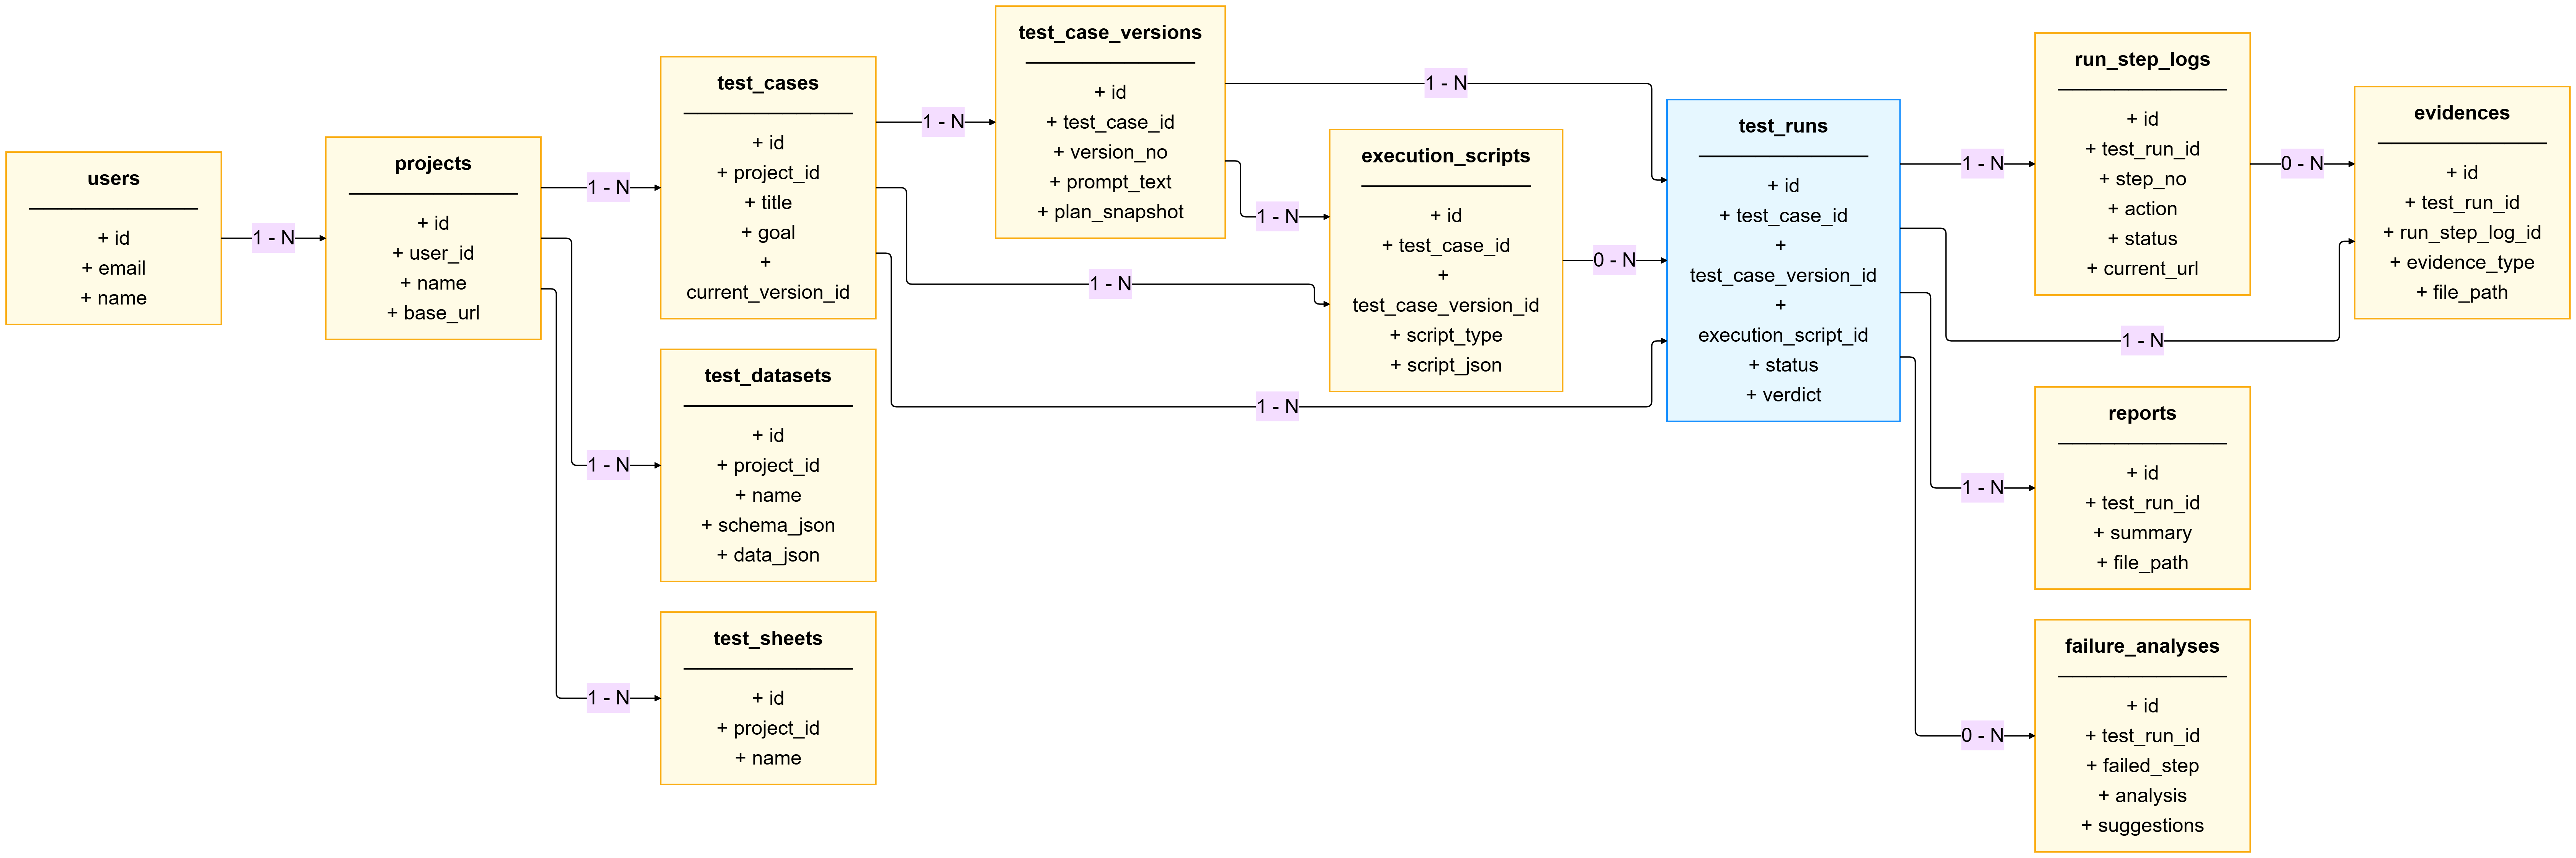
\includegraphics[
        width=\textwidth,
        height=0.78\textheight,
        keepaspectratio
    ]{images/chapter4/db_core_lifecycle.png}
    \caption{Mô hình dữ liệu cốt lõi phục vụ vòng đời kiểm thử}
    \label{fig:db_core_lifecycle}
\end{figure}

\begin{table}[H]
\centering
\caption{Các bảng cốt lõi trong thiết kế dữ liệu}
\label{tab:chapter4_core_tables}
\renewcommand{\arraystretch}{1.2}
\begin{tabular}{|p{3.4cm}|p{5.0cm}|p{5.8cm}|}
\hline
\textbf{Bảng} &
\textbf{Vai trò chính} &
\textbf{Ý nghĩa trong vòng đời kiểm thử} \\
\hline

\texttt{users} &
Lưu thông tin người dùng đã xác thực. &
Liên kết project và các hoạt động kiểm thử với tester. \\
\hline

\texttt{projects} &
Lưu project, base URL và cấu hình liên quan. &
Là đơn vị tổ chức chính của dữ liệu kiểm thử. \\
\hline

\texttt{test\_cases} &
Lưu tên, mục tiêu, trạng thái, vị trí thư mục và thông tin tổng quát của test case chính thức. &
Mô tả nghiệp vụ cần kiểm thử và quản lý test case trong cây thư mục. \\
\hline

\shortstack[l]{\texttt{test\_case\_}\\\texttt{versions}} &
Lưu prompt, goal, Test Plan và nội dung theo từng phiên bản. &
Cho phép truy vết nội dung test case tại thời điểm chạy. \\
\hline

\shortstack[l]{\texttt{execution\_}\\\texttt{scripts}} &
Lưu replay script được tạo từ lịch sử chạy agent. &
Hỗ trợ kiểm thử hồi quy mà không cần agent suy luận lại ở từng bước. \\
\hline

\texttt{test\_runs} &
Lưu trạng thái, verdict, thời gian và lỗi tổng quát của mỗi lần chạy. &
Đại diện cho một lần thực thi cụ thể. \\
\hline

\texttt{run\_step\_logs} &
Lưu trạng thái và thông tin theo từng step. &
Hỗ trợ xác định bước thành công hoặc thất bại. \\
\hline

\texttt{evidences} &
Lưu screenshot, log file, artifact hoặc metadata evidence. &
Cung cấp bằng chứng để kiểm chứng và phân tích kết quả. \\
\hline
\end{tabular}
\end{table}

Trong mô hình trên, \texttt{projects} là thực thể gốc để gom nhóm dữ liệu. \texttt{test\_cases} và \texttt{test\_case\_versions} mô tả nội dung kiểm thử; \texttt{execution\_scripts} lưu replay script; còn \texttt{test\_runs}, \texttt{run\_step\_logs} và \texttt{evidences} lưu dữ liệu thực thi.

% ---------------------------------------------------------
\subsection{Các nhóm bảng hỗ trợ}

Ngoài các bảng cốt lõi, hệ thống sử dụng các nhóm bảng hỗ trợ cho lịch sử sinh test case, test suite, dataset, phân tích lỗi, Object Repository và cấu hình vận hành.

\begin{table}[H]
\centering
\caption{Các nhóm bảng hỗ trợ trong hệ thống}
\label{tab:chapter4_support_tables}
\renewcommand{\arraystretch}{1.2}
\begin{tabular}{|p{3.8cm}|p{5.2cm}|p{5.2cm}|}
\hline
\textbf{Nhóm bảng hỗ trợ} &
\textbf{Ví dụ bảng} &
\textbf{Vai trò tổng quan} \\
\hline

Lịch sử sinh bằng AI &
Các bảng generation batch và candidate &
Lưu từng lần sinh và các test case đề xuất tại trang \textit{Generate Testcase}. Candidate chỉ được chuyển thành test case chính thức sau khi được tester lựa chọn và hoàn tất quá trình tạo script. \\
\hline

Báo cáo và phân tích &
\texttt{reports}, \texttt{failure\_analyses} &
Lưu báo cáo kết quả và nội dung phân tích bằng AI. \\
\hline

Dữ liệu kiểm thử &
\texttt{test\_datasets} và các bảng dữ liệu liên quan &
Lưu dataset và kết quả chạy theo từng dòng dữ liệu. \\
\hline

Test suite &
\texttt{test\_sheets}, \texttt{test\_sheet\_runs} &
Hiện thực test suite, cấu hình chạy theo nhóm và kết quả tổng hợp. \\
\hline

Object Repository &
Các bảng object, selector collection và attribute snapshot &
Lưu thông tin nhận diện phần tử để hỗ trợ tái sử dụng và locator fallback. \\
\hline

Cấu hình runtime &
\texttt{agent\_runtime\_configs}, \texttt{browser\_profiles} &
Lưu timeout, allowed domains, cấu hình trình duyệt và tham số thực thi. \\
\hline

Xác thực và phiên làm việc &
\texttt{sessions}, \texttt{project\_secrets} &
Quản lý phiên đăng nhập, dữ liệu nhạy cảm và thông tin xác thực. \\
\hline
\end{tabular}
\end{table}

Tên bảng vật lý \texttt{test\_sheets} được sử dụng để hiện thực chức năng test suite trên giao diện. Trong nội dung báo cáo, thuật ngữ \textit{test suite} được dùng thống nhất khi nói về chức năng nghiệp vụ.

% ---------------------------------------------------------
\subsection{Các quyết định schema đáng chú ý}

\begin{table}[H]
\centering
\caption{Các quyết định schema đáng chú ý}
\label{tab:chapter4_schema_decisions}
\renewcommand{\arraystretch}{1.2}
\begin{tabular}{|p{4.2cm}|p{10.0cm}|}
\hline
\textbf{Quyết định} &
\textbf{Lý do} \\
\hline

Chỉ trình bày bảng cốt lõi trong ERD chính &
Giữ mô hình tập trung vào vòng đời kiểm thử và tránh làm sơ đồ quá phức tạp. \\
\hline

Tách test case đề xuất và test case chính thức &
Test case do AI sinh ban đầu được lưu dưới dạng candidate. Chỉ những candidate được tester lựa chọn và hoàn tất quá trình tạo script mới được đưa vào kho test case chính thức. \\
\hline

Tách test case và test run &
Một test case có thể được chạy nhiều lần và tạo ra các kết quả khác nhau. \\
\hline

Quản lý test case theo phiên bản &
Cho phép truy vết nội dung test case tại thời điểm mỗi test run được tạo. \\
\hline

Lưu replay script dạng JSON &
Hỗ trợ nhiều loại action, assertion, tham số và metadata có cấu trúc linh hoạt. \\
\hline

Tổ chức test case theo cây thư mục &
Giúp tester phân nhóm và quản lý test case theo chức năng, module hoặc luồng nghiệp vụ. \\
\hline

Tách evidence khỏi test run &
Một test run có thể có nhiều screenshot, log và artifact khác nhau. \\
\hline

Lưu snapshot khi thực thi &
Giữ lại cấu hình runtime, replay script hoặc dataset tại thời điểm chạy. \\
\hline

Sử dụng JSON/JSONB &
Phù hợp với replay script, action history, selector collection và evidence summary có cấu trúc linh hoạt. \\
\hline
\end{tabular}
\end{table}

Các tiến trình bất đồng bộ như scan, generation batch, test run, replay run và suite run sử dụng các trạng thái như \texttt{pending}, \texttt{running}, \texttt{passed}, \texttt{failed}, \texttt{error} và \texttt{cancelled} tùy theo loại tiến trình.

% =========================================================
\section{Thiết kế các luồng xử lý cốt lõi}
% =========================================================

Các luồng xử lý được tổ chức theo vòng đời kiểm thử: tạo project, sinh và lựa chọn test case, tạo script bằng agent, xác nhận replay script, chạy kiểm thử hồi quy và lưu kết quả.

% ---------------------------------------------------------
\subsection{Luồng tạo project và scan/crawl website}

Tester khai báo tên project, mô tả, base URL và cấu hình liên quan. Backend kiểm tra dữ liệu, tạo project và xác định phạm vi website mục tiêu.

Sau khi tạo project, tester có thể khởi tạo scan/crawl để thu thập sitemap và interaction map. Đây là bước tùy chọn nhằm cung cấp thêm ngữ cảnh cho quá trình sinh test case và chạy agent.

% ---------------------------------------------------------
\subsection{Luồng sinh và lựa chọn test case}

Tester truy cập trang \textit{Generate Testcase} và nhập yêu cầu, mục tiêu hoặc mô tả chức năng cần kiểm thử bằng ngôn ngữ tự nhiên. Backend kết hợp nội dung này với thông tin project và dữ liệu scan nếu có, sau đó gọi LLM để sinh danh sách test case đề xuất gồm tiêu đề, mục tiêu, Test Plan, dữ liệu đầu vào và kết quả kỳ vọng.

Các test case được hiển thị trong khu vực làm việc để tester xem xét, chỉnh sửa và lựa chọn. Những test case chưa được lựa chọn chỉ là kết quả đề xuất và chưa được đưa vào kho test case chính thức của project.

Các test case được lựa chọn tiếp tục được sử dụng làm đầu vào cho agent nhằm tạo automation test script. Sau khi script được tạo thành công và được tester xác nhận, test case cùng replay script được chuyển sang trang \textit{Test Cases} để lưu trữ theo cấu trúc cây thư mục.

\begin{figure}[H]
    \centering
    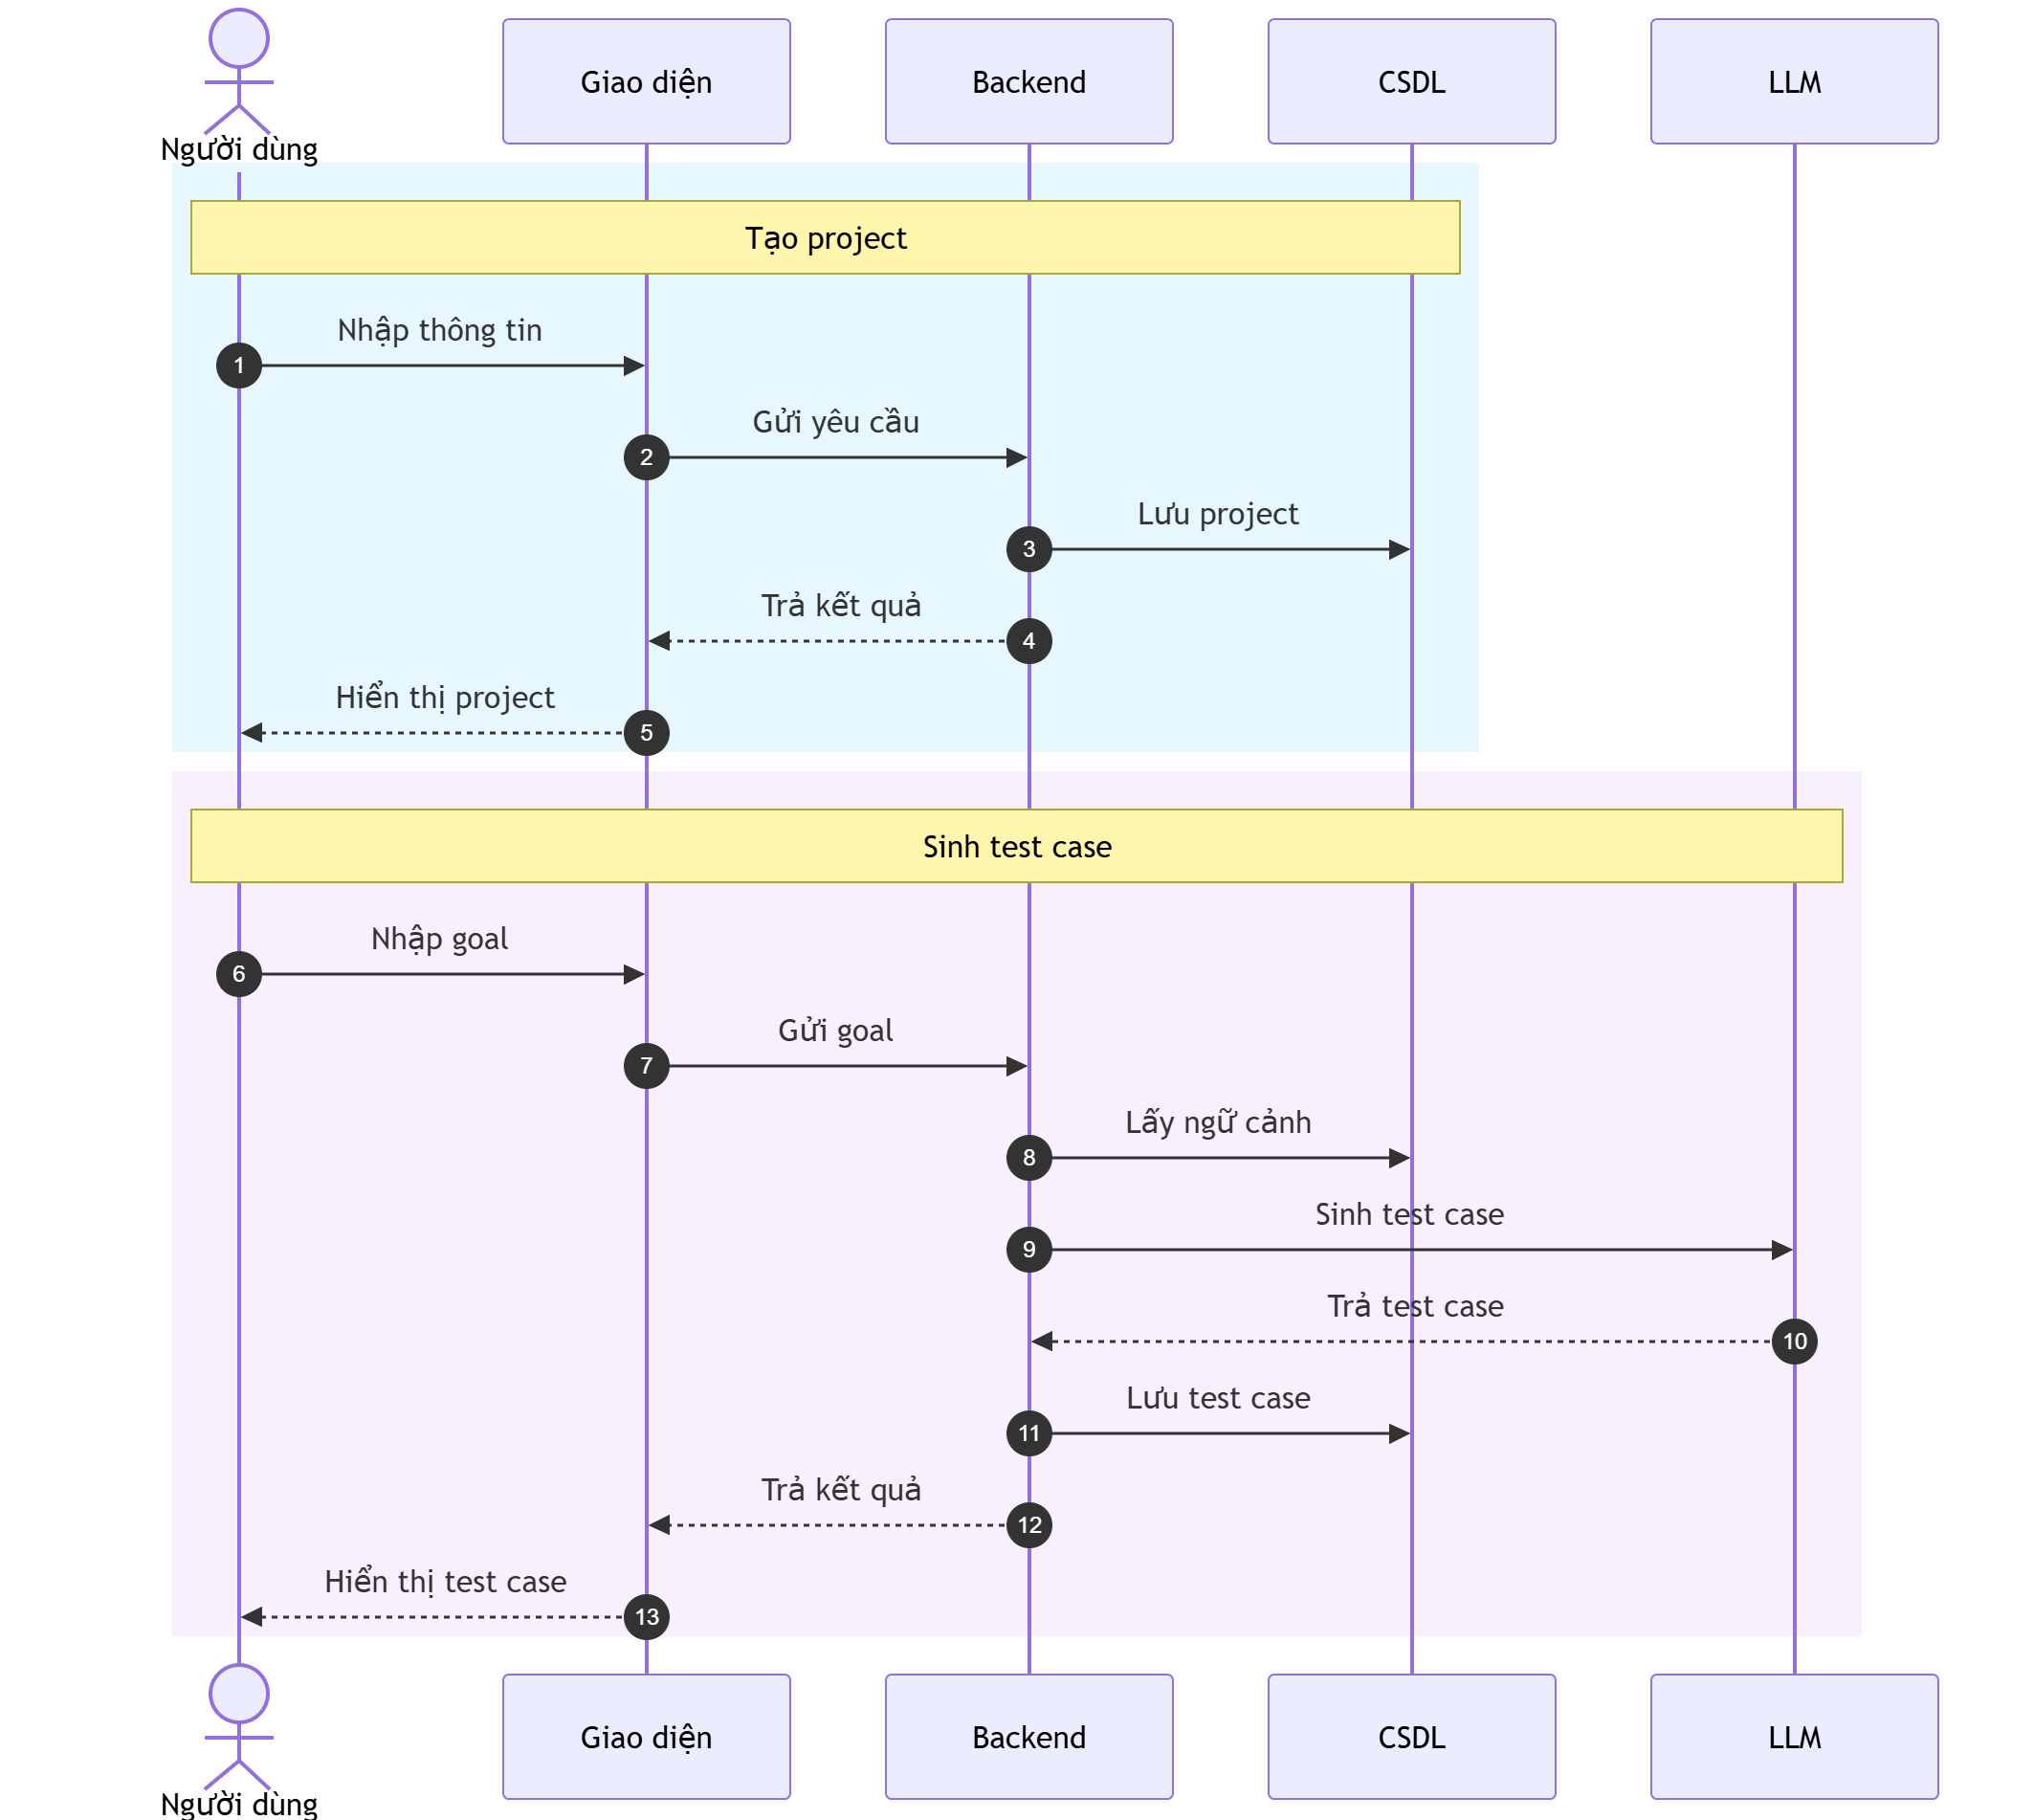
\includegraphics[
        width=\textwidth,
        height=0.78\textheight,
        keepaspectratio
    ]{images/chapter4/flow_project_testcase_creation.png}
    \caption{Luồng tạo project, sinh, lựa chọn test case và tạo test script}
    \label{fig:flow_project_testcase_creation}
\end{figure}

% ---------------------------------------------------------
\subsection{Luồng tạo test script bằng goal-based agent}

Agent được sử dụng trong giai đoạn thực thi ban đầu để khám phá giao diện và tạo automation test script từ test case đã được tester lựa chọn.

\begin{figure}[H]
    \centering
    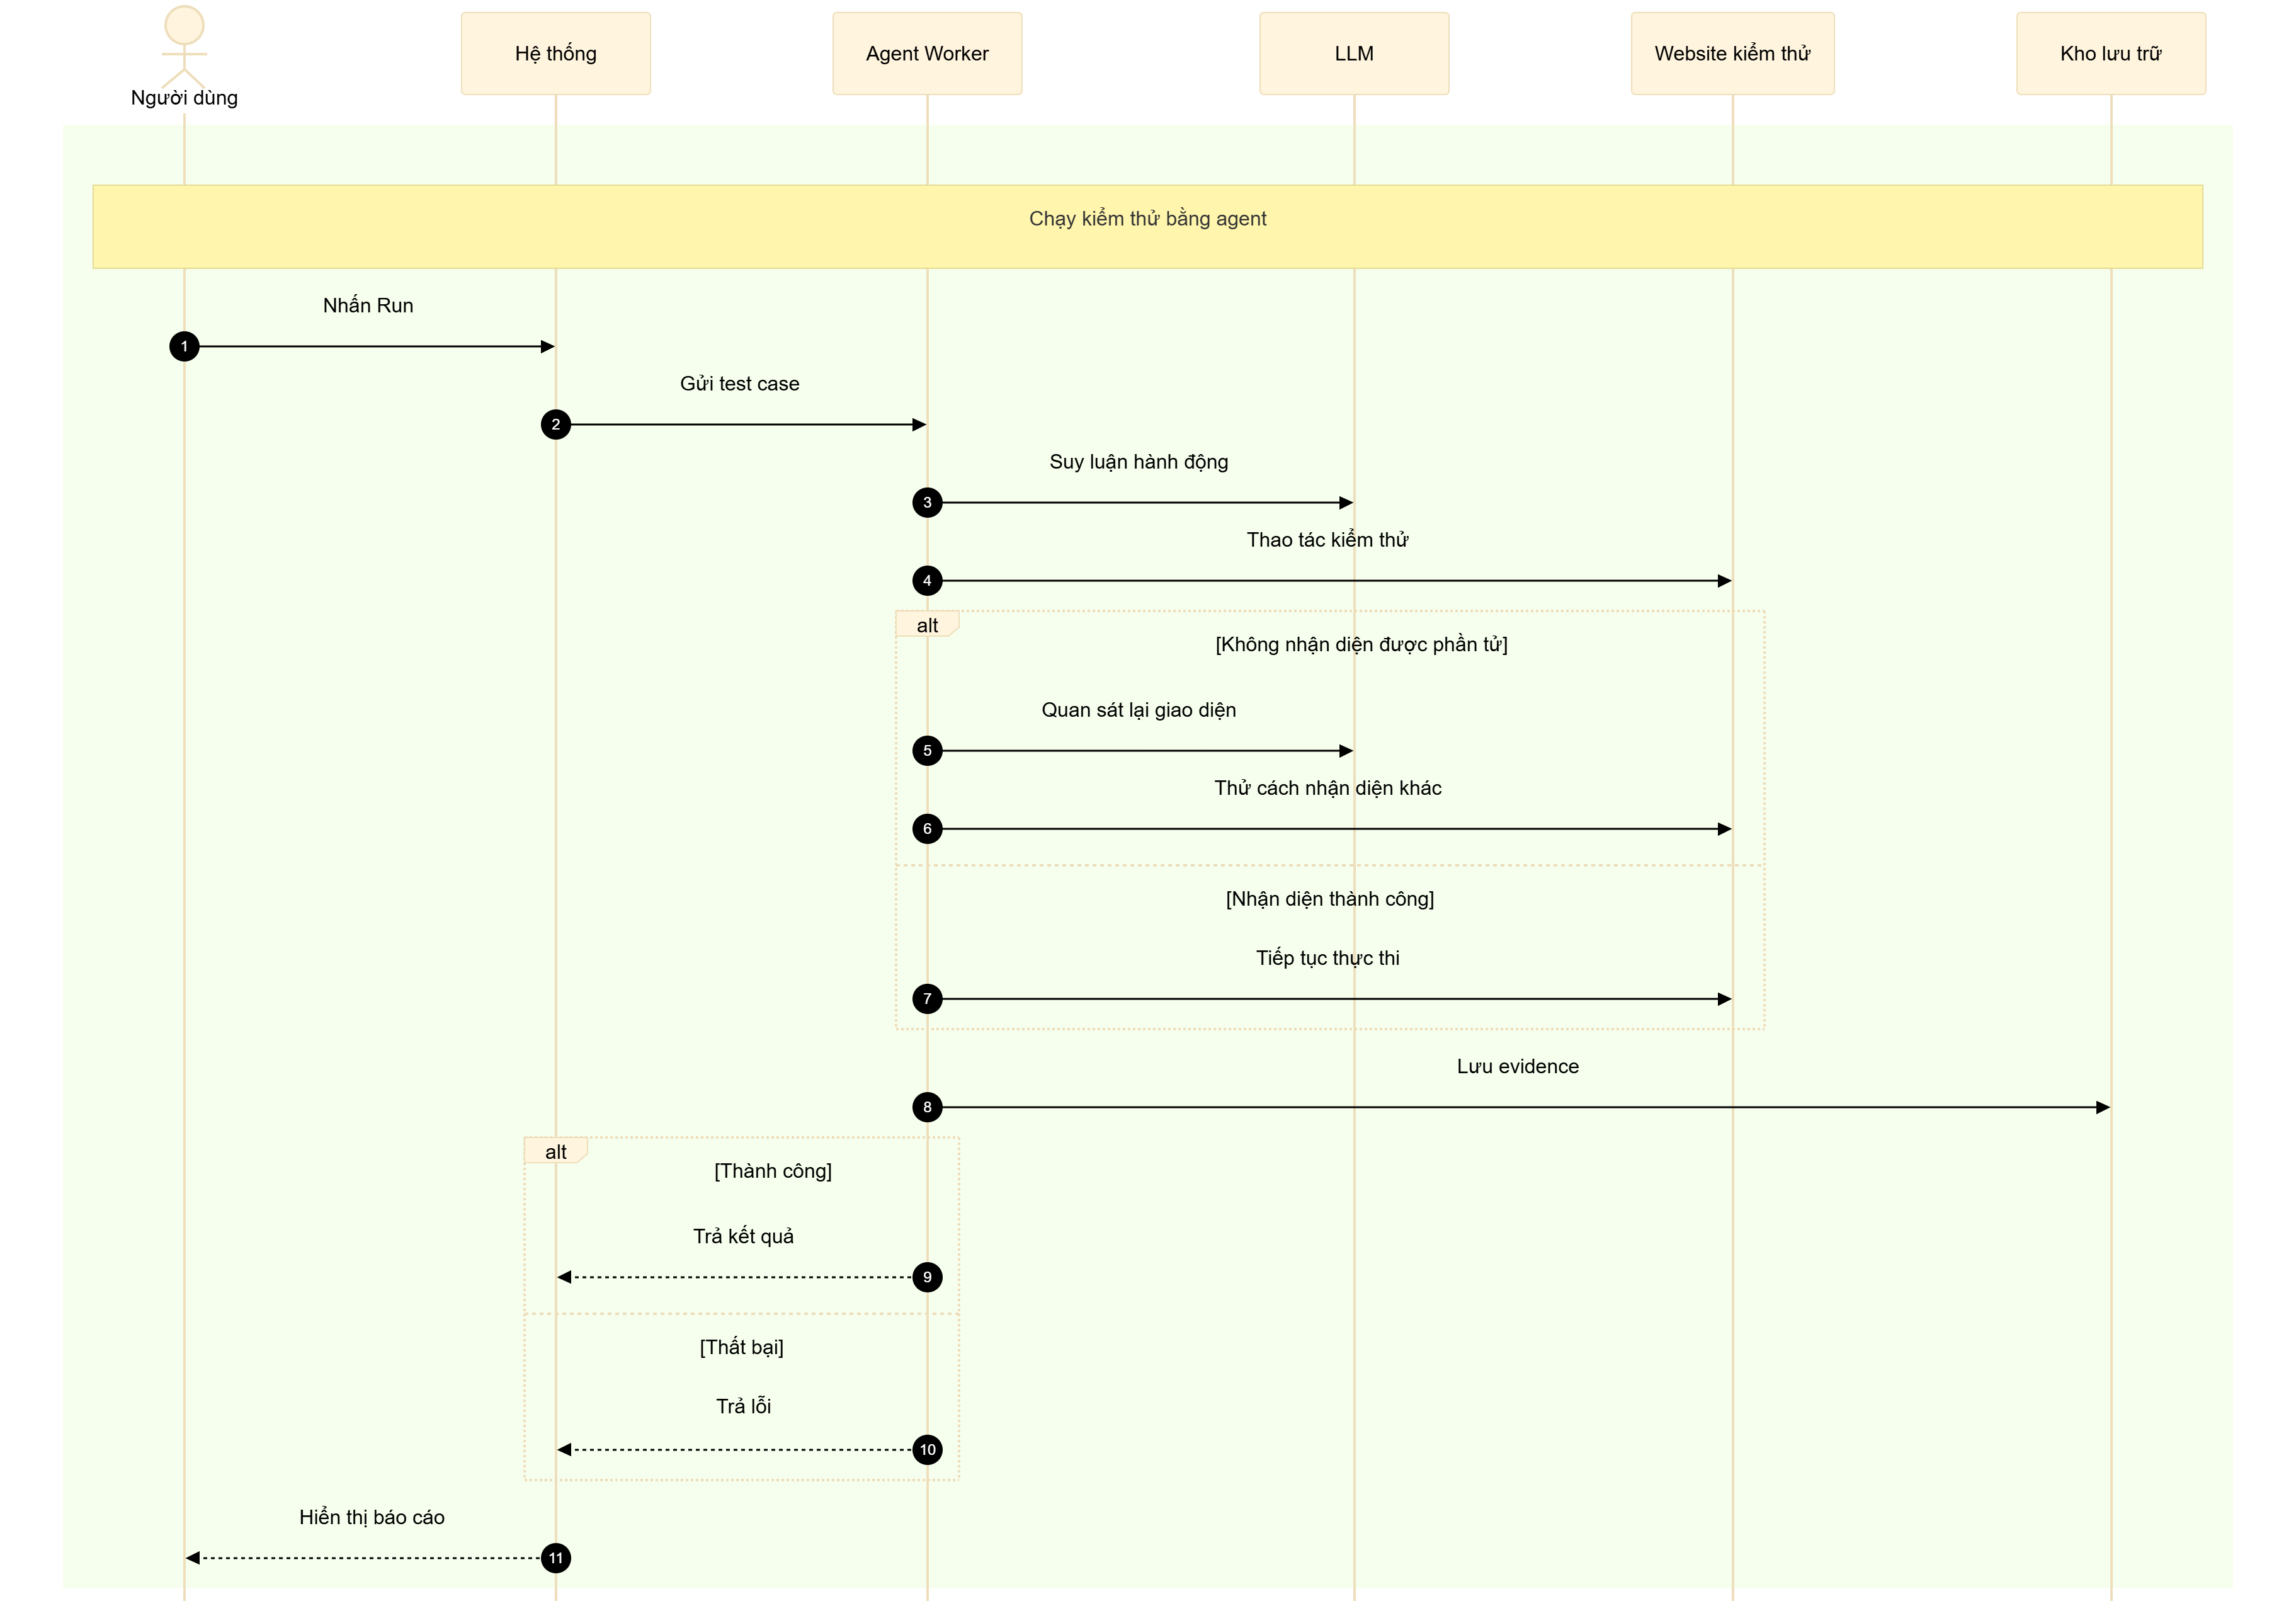
\includegraphics[
        width=\textwidth,
        height=0.78\textheight,
        keepaspectratio
    ]{images/chapter4/flow_agent_test_execution.png}
    \caption{Luồng tạo automation test script bằng goal-based agent}
    \label{fig:flow_agent_test_execution}
\end{figure}

Backend tạo test run và gửi test case cùng cấu hình thực thi sang agent-worker. Worker khởi tạo trình duyệt, sử dụng agent và LLM để quan sát giao diện, suy luận và thực hiện action.

Trong quá trình chạy, worker ghi nhận step log, screenshot, action history và evidence. Nếu cách nhận diện phần tử ban đầu không còn phù hợp, agent có thể quan sát lại giao diện hoặc sử dụng thông tin trong Object Repository để thử cách định vị khác.

Khi phiên chạy thành công, action history được chuẩn hóa thành replay script. Tester xem xét kết quả trước khi xác nhận script và đưa test case vào kho test case chính thức.

% ---------------------------------------------------------
\subsection{Luồng chạy bằng replay script}

Replay script được sử dụng khi test case đã có kịch bản được xác nhận. Chế độ này ưu tiên tính ổn định, khả năng lặp lại và phù hợp với kiểm thử hồi quy.

\begin{figure}[H]
    \centering
    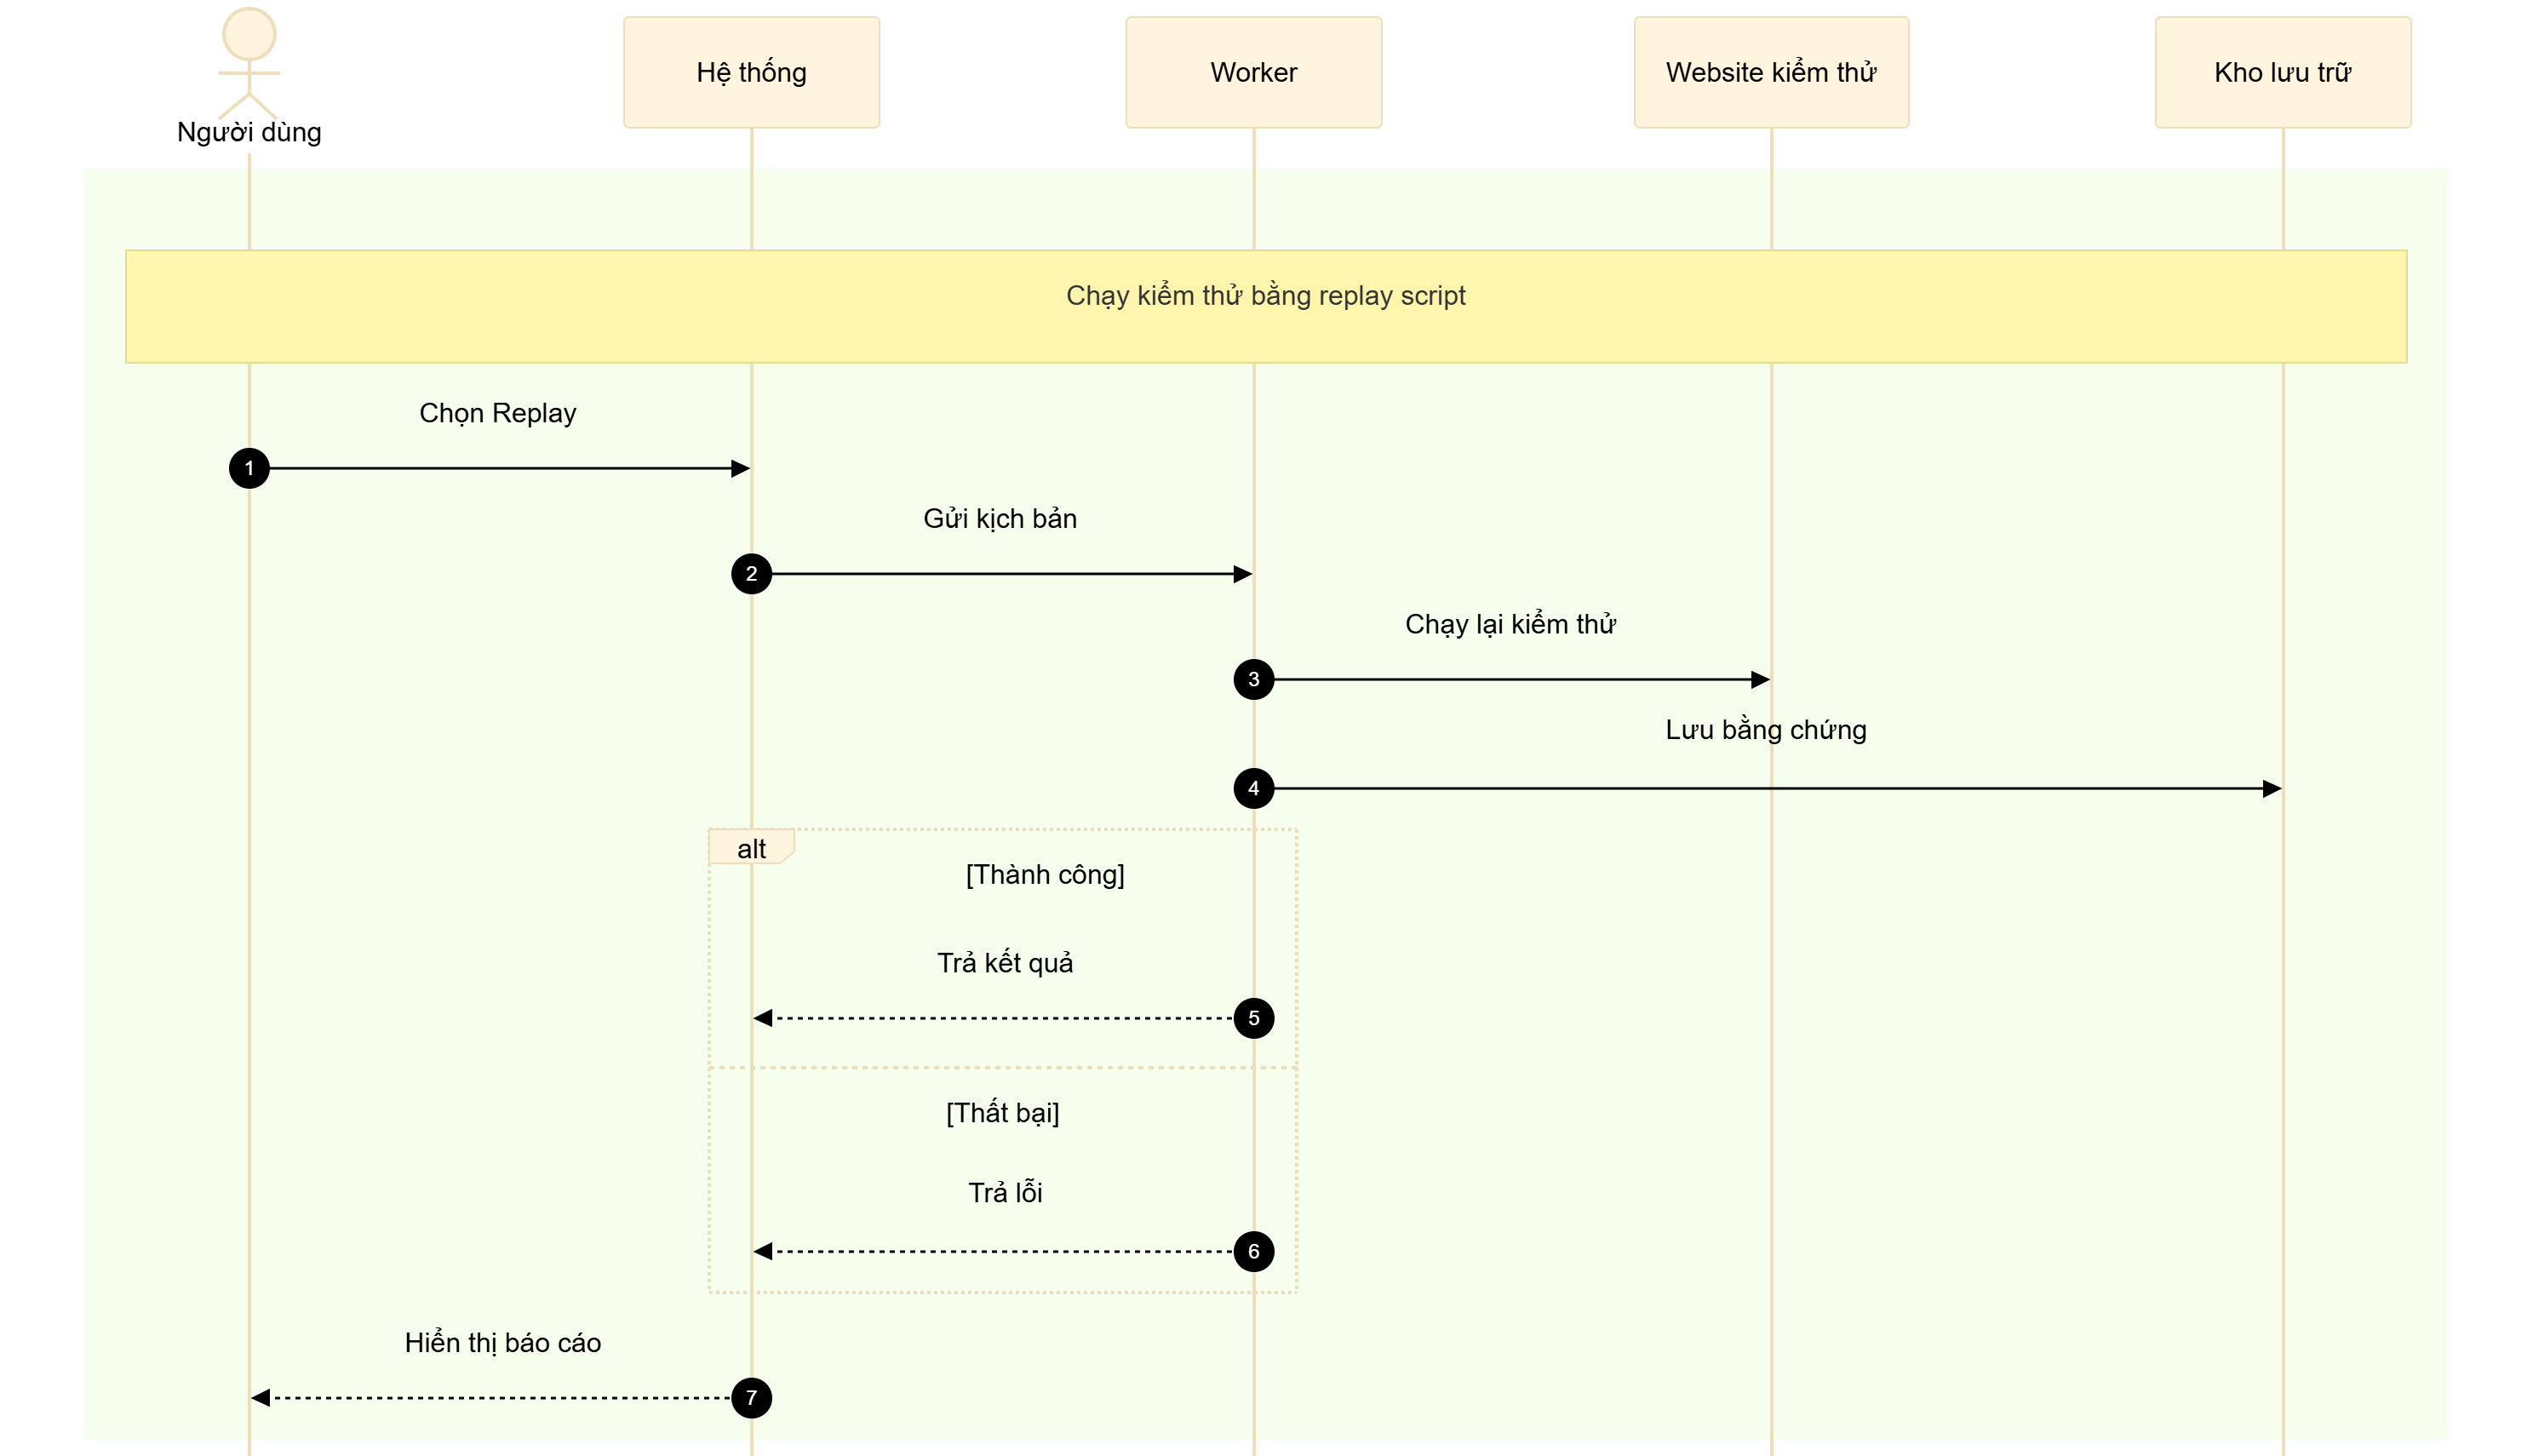
\includegraphics[
        width=\textwidth,
        height=0.78\textheight,
        keepaspectratio
    ]{images/chapter4/flow_replay_execution.png}
    \caption{Luồng chạy test case bằng replay script}
    \label{fig:flow_replay_execution}
\end{figure}

Agent-worker đọc replay script và thực thi các step theo thứ tự bằng thành phần tự động hóa trình duyệt. Replay script không yêu cầu LLM suy luận lại ở từng bước.

Khi được chạy với dataset, các biến trong script được thay thế bằng dữ liệu của từng dòng. Nếu locator, action hoặc assertion không còn phù hợp, hệ thống ghi nhận trạng thái \texttt{failed} hoặc \texttt{error} và lưu evidence để phân tích.

Nếu website thay đổi đáng kể làm replay script không còn phù hợp, tester có thể cập nhật script hoặc sử dụng agent để tạo lại kịch bản.

% ---------------------------------------------------------
\subsection{Luồng lưu evidence và sinh report}

Trong quá trình chạy, agent-worker ghi nhận trạng thái step, URL, screenshot, action history và log kỹ thuật. Khi kết thúc, worker gửi verdict, error message và evidence summary về backend.

\begin{figure}[H]
    \centering
    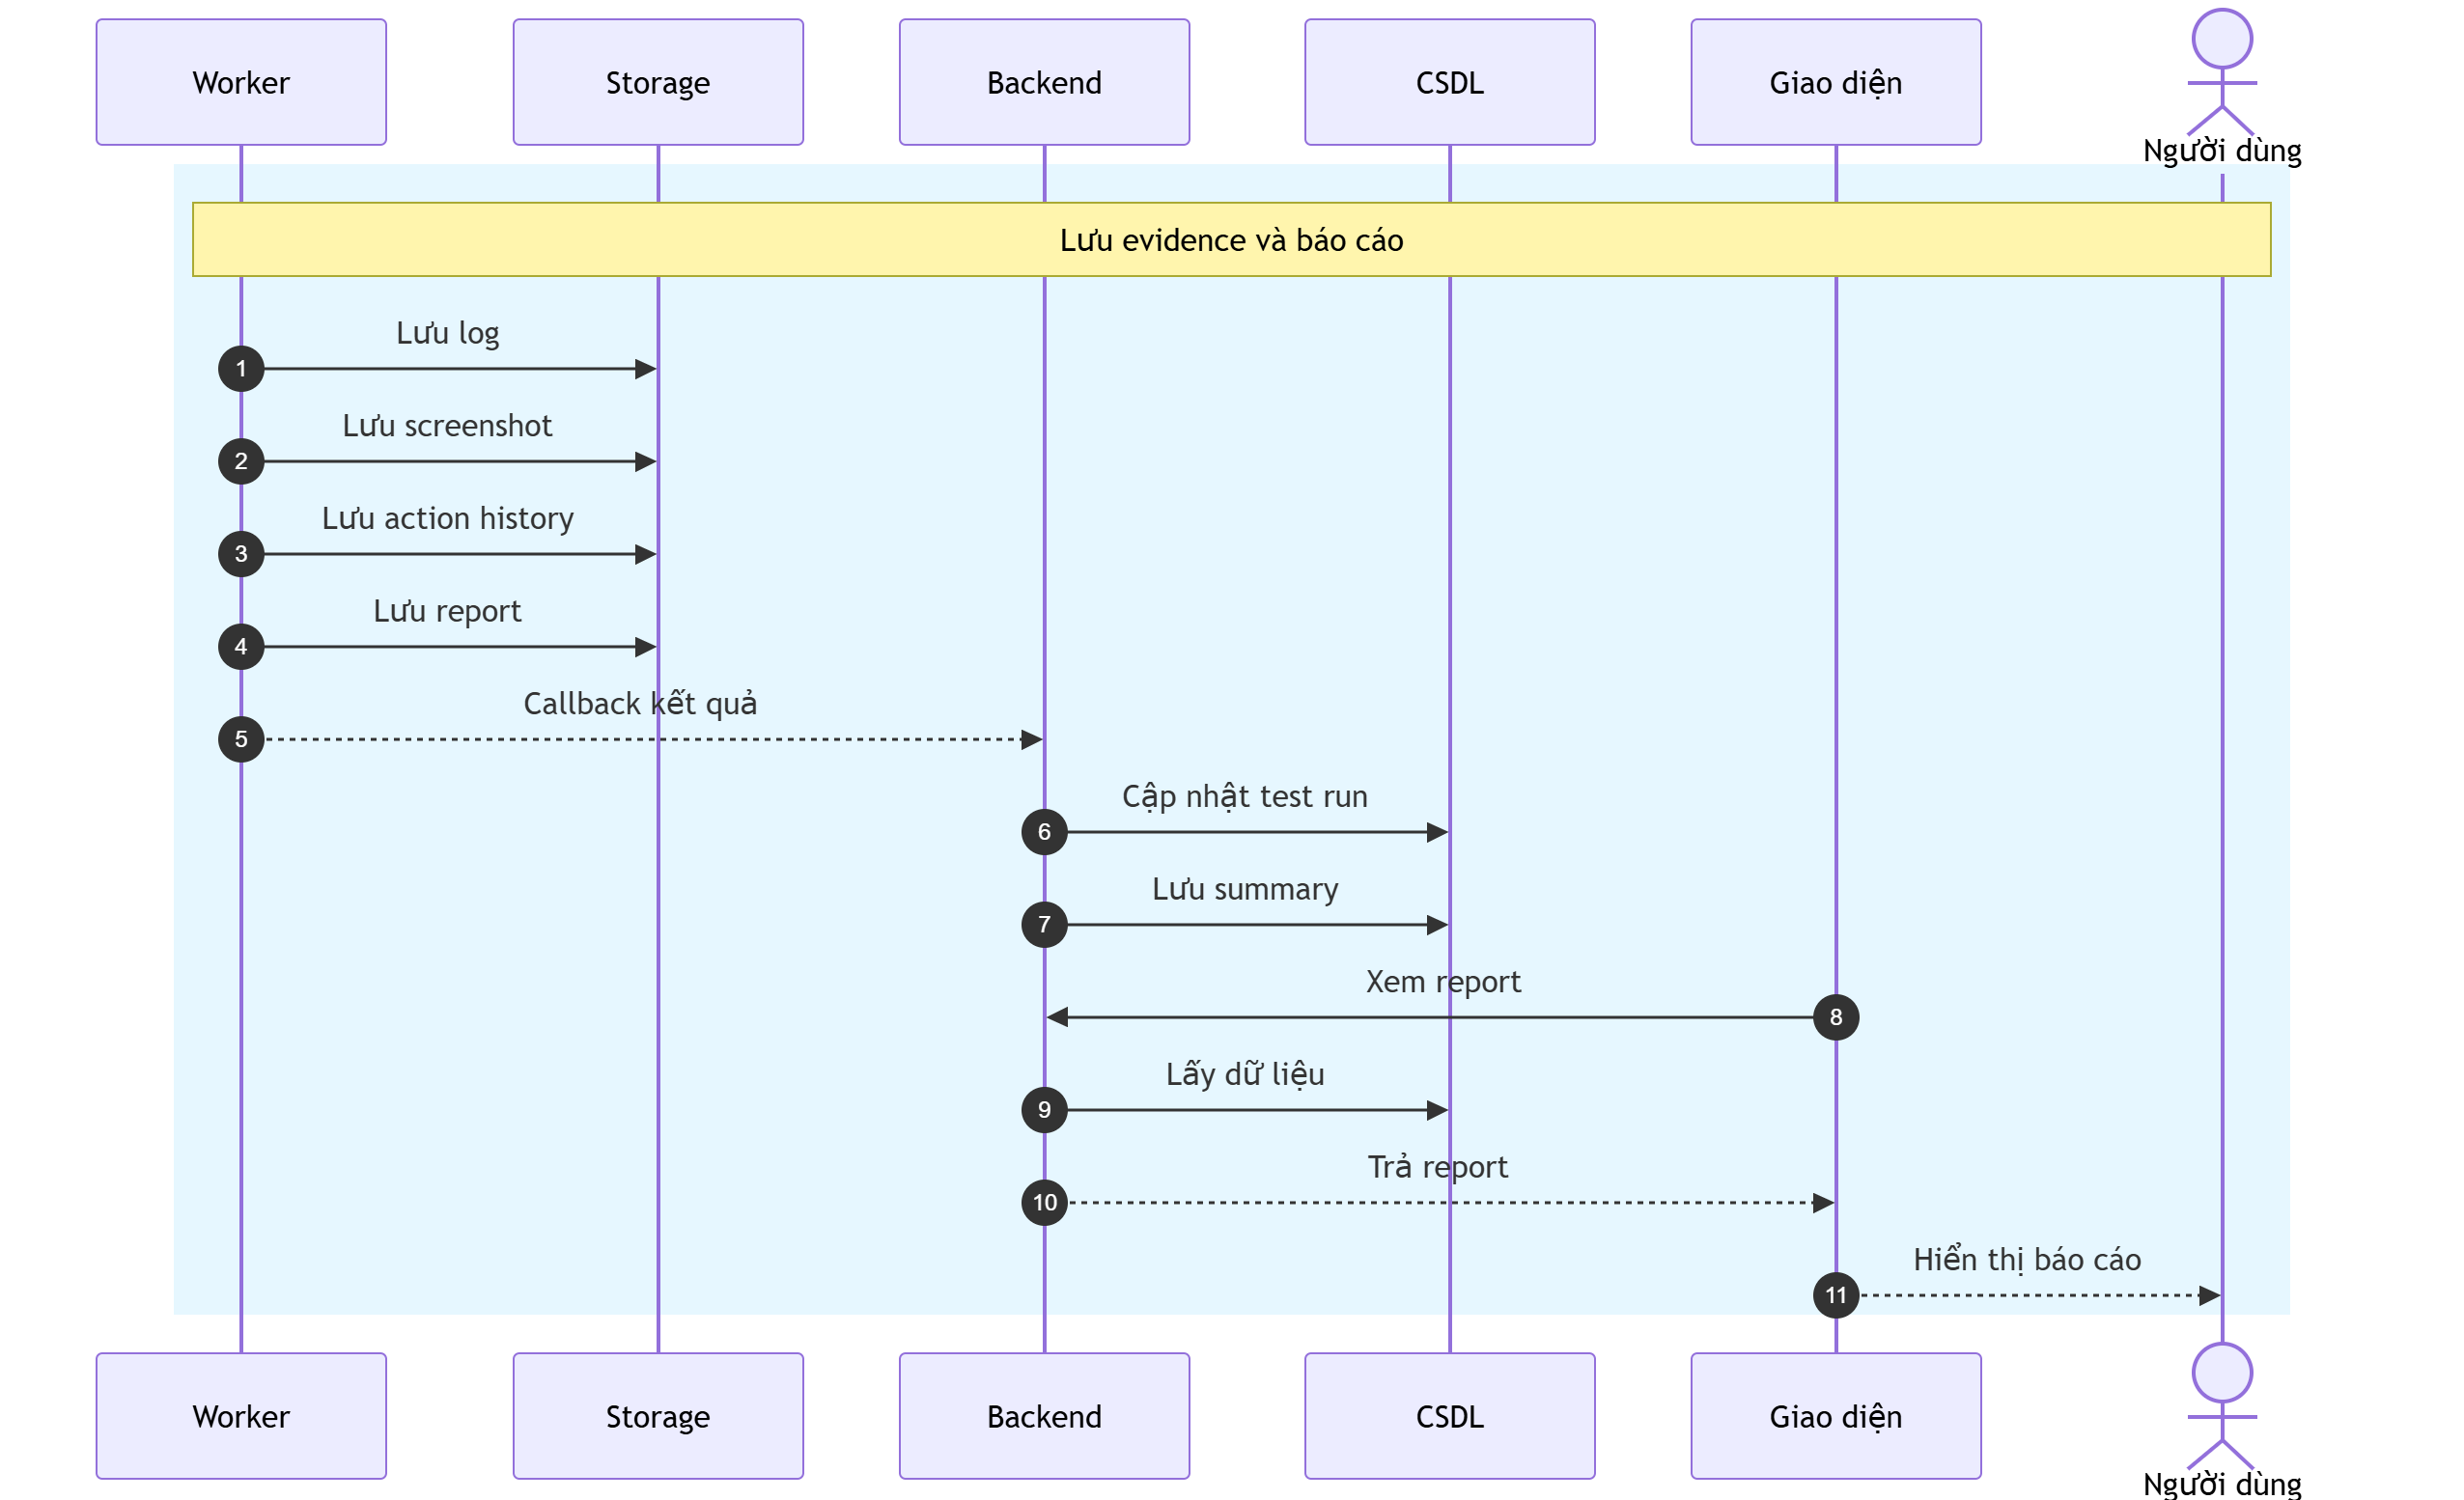
\includegraphics[
        width=\textwidth,
        height=0.78\textheight,
        keepaspectratio
    ]{images/chapter4/flow_report_evidence.png}
    \caption{Luồng lưu evidence và sinh báo cáo kết quả}
    \label{fig:flow_report_evidence}
\end{figure}

Backend cập nhật test run, lưu evidence và cung cấp dữ liệu cho giao diện. Report hiển thị trạng thái, timeline, screenshot và thông tin lỗi. Log kỹ thuật được lưu để hỗ trợ AI Analysis và truy vết khi cần.

% =========================================================
\section{Thiết kế agent-worker và cơ chế thực thi}
% =========================================================

Agent-worker là thành phần trực tiếp khởi tạo trình duyệt, chạy agent hoặc replay script và ghi nhận evidence. Việc tách worker khỏi backend giúp backend tập trung vào nghiệp vụ, trong khi worker xử lý các tác vụ tiêu tốn nhiều tài nguyên.

\begin{figure}[H]
    \centering
    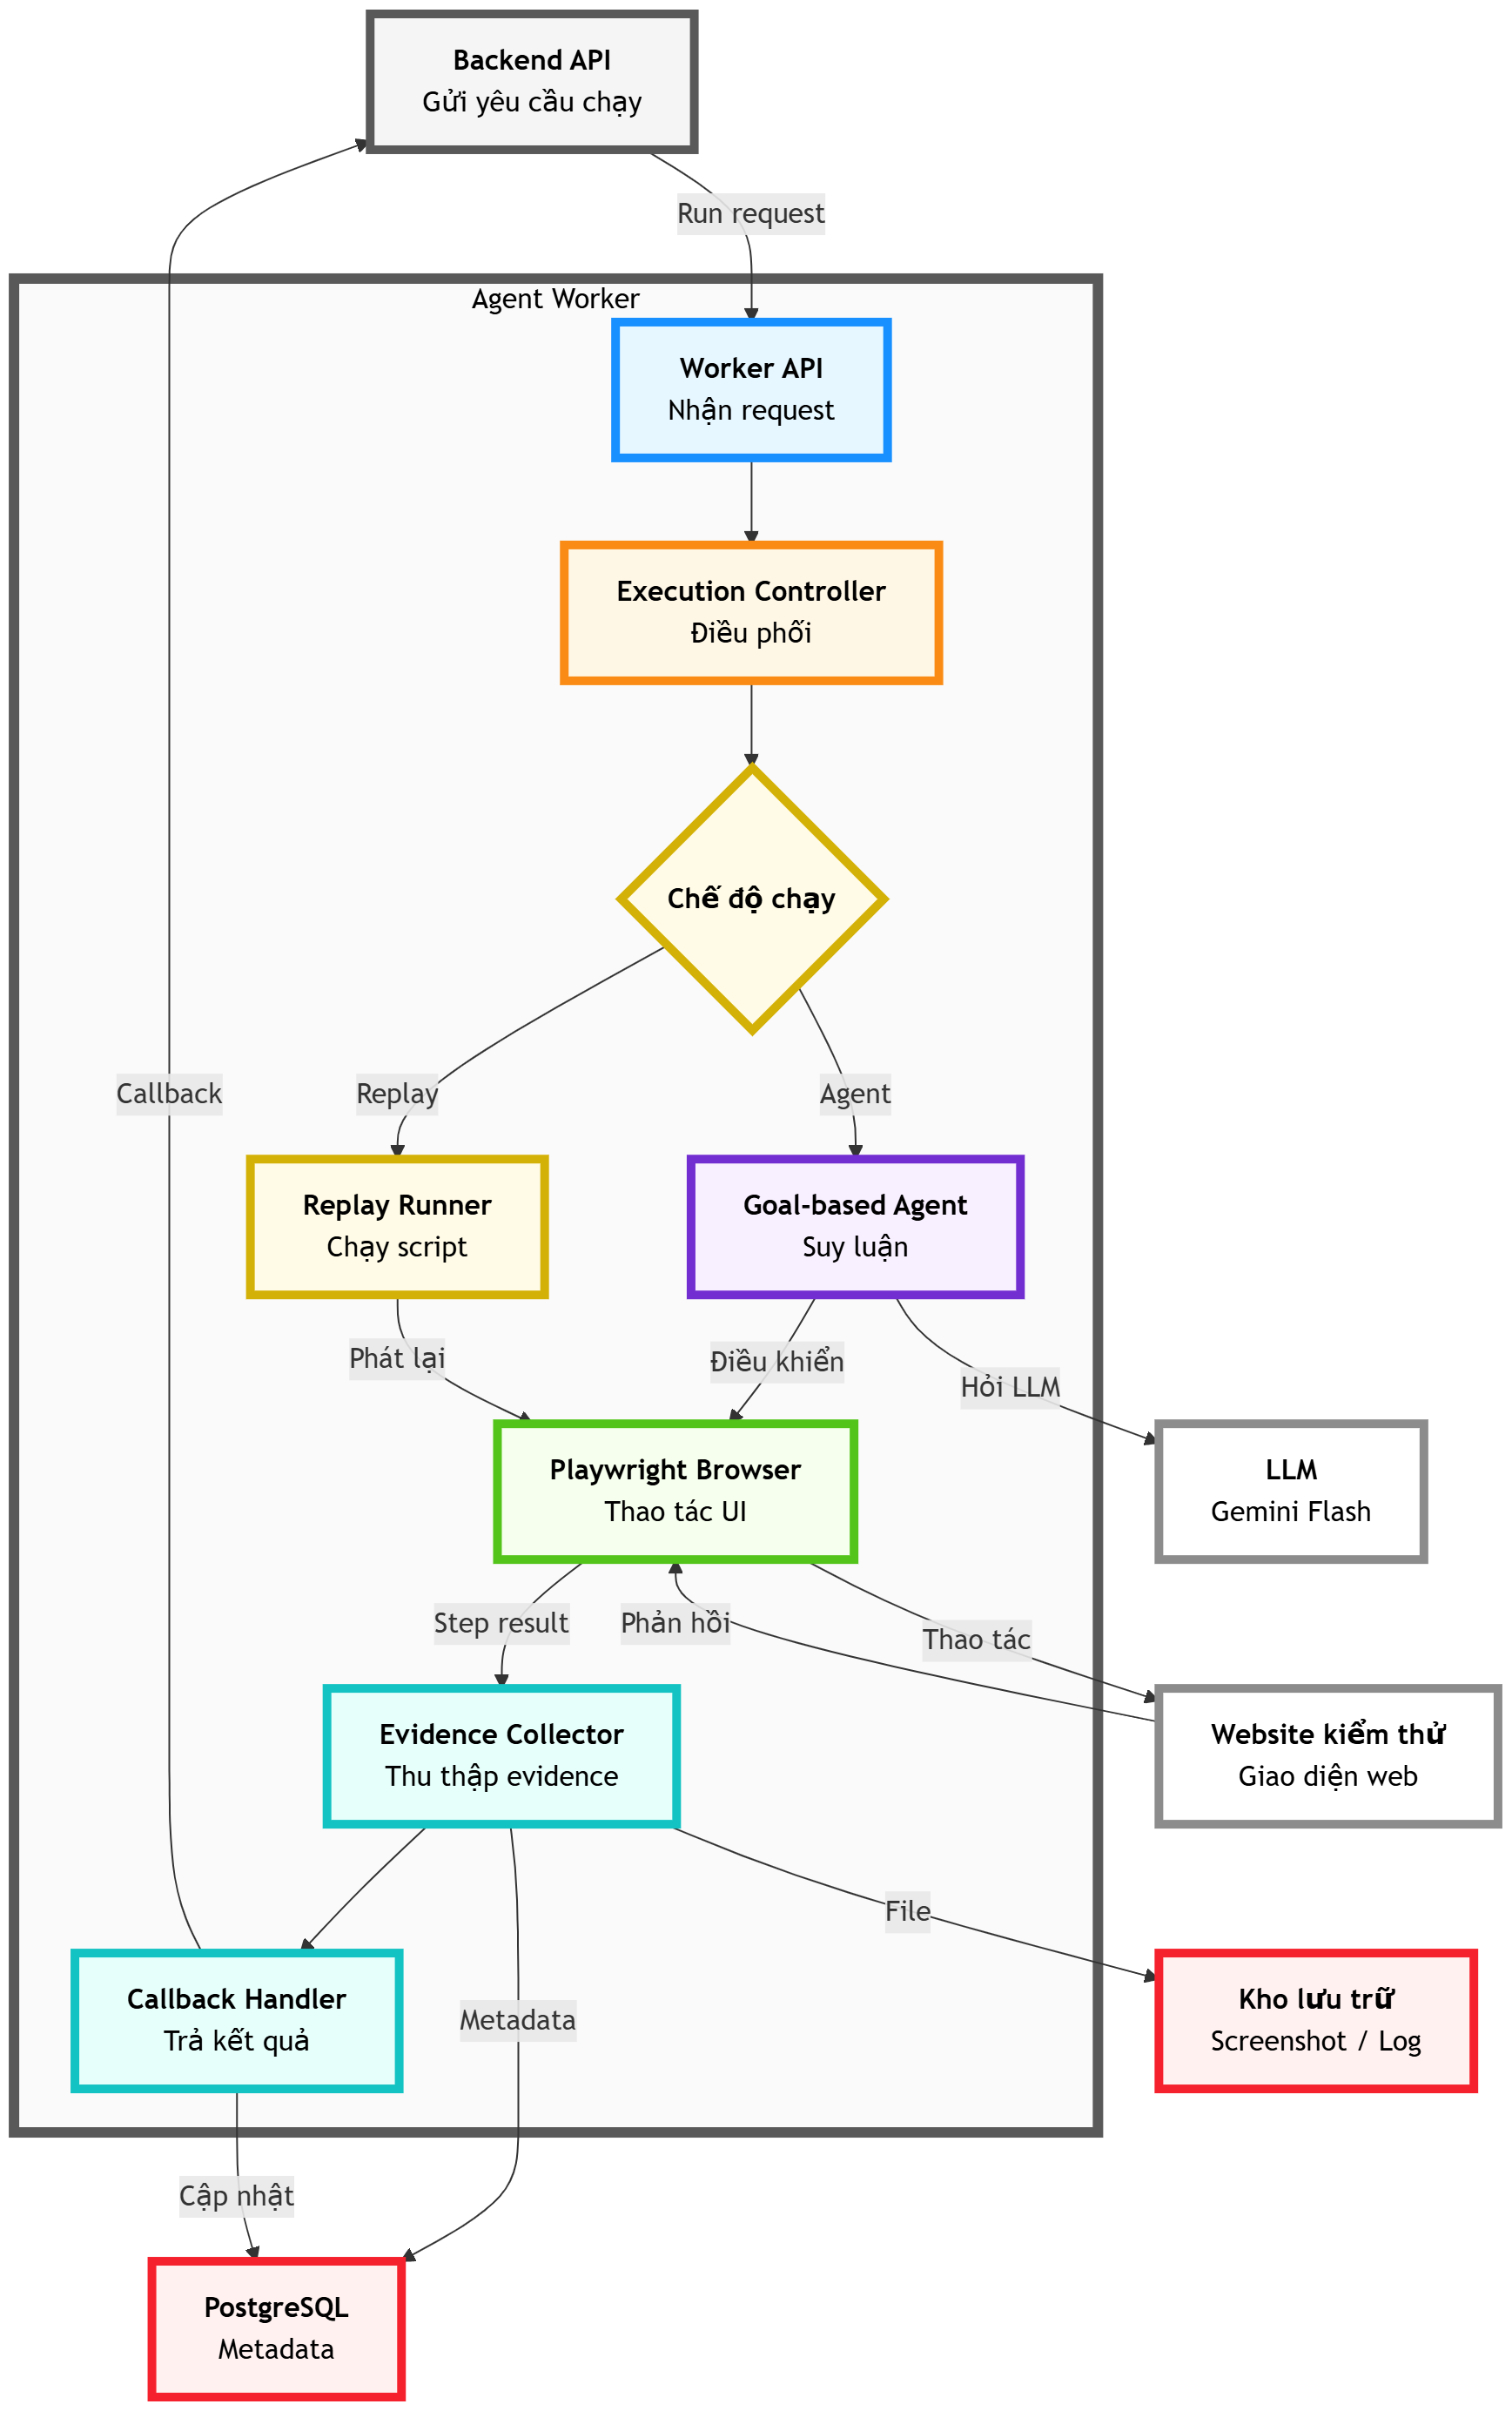
\includegraphics[
        width=\textwidth,
        height=0.78\textheight,
        keepaspectratio
    ]{images/chapter4/agent_worker_design.png}
    \caption{Thiết kế bên trong agent-worker}
    \label{fig:agent_worker_design}
\end{figure}

Trong chế độ agent, worker nhận goal, Test Plan, dữ liệu đầu vào và cấu hình runtime. Worker phối hợp LLM với thành phần tự động hóa trình duyệt để quan sát giao diện, thực hiện action và kiểm tra trạng thái.

Chế độ agent chủ yếu được sử dụng để tạo automation test script ban đầu hoặc tạo lại script khi website thay đổi đáng kể.

Trong chế độ replay, worker đọc replay script và phát lại các action theo thứ tự. Chế độ này không cần LLM suy luận ở từng bước, giúp giảm chi phí và tăng tính lặp lại của kết quả.

Agent-worker cần kiểm soát timeout, số phiên trình duyệt đồng thời, allowed domains và các lỗi như website không tải được, locator thất bại hoặc assertion không đạt.

% =========================================================
\section{Thiết kế cơ chế hỗ trợ bảo trì kiểm thử}
% =========================================================

\subsection{Object Repository và State Anchors}

Object Repository lưu thông tin nhận diện phần tử theo project. Mỗi object có thể gồm tên, page key, selector collection, attribute snapshot và nguồn tạo. Dữ liệu này hỗ trợ tái sử dụng selector giữa nhiều replay script.

State Anchors là các điều kiện xác nhận trạng thái quan trọng, chẳng hạn URL thay đổi, phần tử xuất hiện, input có giá trị đúng hoặc thông báo lỗi được hiển thị. Các anchor hoặc assertion được sử dụng để xác định verdict của test case.

Locator fallback được sử dụng khi locator ban đầu không còn phù hợp. Thành phần thực thi có thể thử selector mặc định, selector dự phòng hoặc thông tin thuộc tính đã lưu trong Object Repository.

Cơ chế này hỗ trợ xử lý các thay đổi nhỏ trên giao diện nhưng không thay thế việc cập nhật test case hoặc tạo lại script khi luồng nghiệp vụ thay đổi đáng kể.

% ---------------------------------------------------------
\subsection{Quản lý test suite và dữ liệu kiểm thử}

Test suite gom nhiều test case đã được lưu trong cây thư mục thành một nhóm chạy. Đối với các test case đã có replay script, hệ thống ưu tiên thực thi bằng replay script để phục vụ kiểm thử hồi quy.

Agent được sử dụng khi test case chưa có script phù hợp hoặc khi cần tạo lại script do website thay đổi đáng kể.

Dữ liệu kiểm thử được lưu thành dataset, trong đó mỗi dòng là một bộ dữ liệu đầu vào. Khi chạy replay script với dataset, hệ thống tạo kết quả riêng cho từng dòng dữ liệu.

Trước khi chạy, hệ thống kiểm tra cấu trúc dataset với các biến của replay script dựa trên tên trường và kiểu dữ liệu. Cấu hình không đầy đủ hoặc dataset không tương thích sẽ bị chặn thực thi.

% =========================================================
\section{Thiết kế bảo mật và kiểm soát vận hành}
% =========================================================

Do hệ thống có khả năng gọi LLM, mở trình duyệt và thao tác trên website mục tiêu, bảo mật và kiểm soát vận hành cần được áp dụng ở tất cả các thành phần.

\begin{table}[H]
\centering
\caption{Các nhóm kiểm soát bảo mật và vận hành}
\label{tab:chapter4_security_operation}
\renewcommand{\arraystretch}{1.2}
\begin{tabular}{|p{4.0cm}|p{10.2cm}|}
\hline
\textbf{Nhóm kiểm soát} &
\textbf{Nội dung thiết kế} \\
\hline

Xác thực và quyền truy cập &
Tester phải đăng nhập; dữ liệu project, test case, dataset, replay script và evidence được kiểm soát theo phạm vi truy cập. \\
\hline

Bảo vệ thông tin xác thực &
Mật khẩu không được lưu dạng thô; API key, token và cấu hình LLM không được gửi xuống frontend. \\
\hline

Bảo vệ backend API &
Backend kiểm tra dữ liệu đầu vào, quyền truy cập project và nguồn của các callback. \\
\hline

Bảo vệ agent-worker &
Worker có timeout, giới hạn phiên trình duyệt đồng thời và chỉ nhận yêu cầu hợp lệ từ backend. \\
\hline

Xác thực callback &
Callback cập nhật step, evidence và kết quả cần có cơ chế xác thực nguồn gửi. \\
\hline

Bảo vệ dữ liệu kiểm thử &
Dataset, screenshot và log có thể chứa dữ liệu nhạy cảm nên cần được kiểm soát quyền truy cập. \\
\hline

Kiểm soát phạm vi website &
Mỗi project xác định base URL và allowed domains để ngăn truy cập ngoài phạm vi kiểm thử. \\
\hline

Kiểm soát prompt injection &
Nội dung website được xem là dữ liệu không tin cậy và không được phép ghi đè quy tắc vận hành của agent~\cite{11359704}. \\
\hline
\end{tabular}
\end{table}

Đối với website yêu cầu đăng nhập, hệ thống nên sử dụng tài khoản test hoặc tài khoản staging có quyền hạn giới hạn.

% =========================================================
\section{Cơ sở lựa chọn thiết kế và các đánh đổi}
% =========================================================

Bảng~\ref{tab:chapter4_design_decisions} tổng hợp các quyết định kiến trúc chính và đánh đổi tương ứng.

\begin{table}[H]
\centering
\caption{Tổng hợp các quyết định kiến trúc lớn}
\label{tab:chapter4_design_decisions}
\renewcommand{\arraystretch}{1.2}
\begin{tabular}{|p{4.0cm}|p{5.2cm}|p{5.0cm}|}
\hline
\textbf{Quyết định} &
\textbf{Lý do chọn} &
\textbf{Đánh đổi} \\
\hline

Tách backend và agent-worker &
Phân tách nghiệp vụ với tác vụ tự động hóa trình duyệt. &
Cần callback và đồng bộ trạng thái giữa hai service. \\
\hline

Tách test case đề xuất và test case chính thức &
Cho phép tester kiểm soát kết quả do AI sinh trước khi đưa vào sử dụng. &
Cần quản lý thêm trạng thái candidate và quá trình xác nhận. \\
\hline

Sử dụng agent để tạo script ban đầu &
Hỗ trợ chuyển test case thành thao tác thực tế mà không yêu cầu tester viết script từ đầu. &
Kết quả có thể không hoàn toàn xác định và phát sinh chi phí LLM. \\
\hline

Kết hợp agent và replay script &
Agent linh hoạt; replay script ổn định và phù hợp hơn với kiểm thử hồi quy. &
Cần chuyển action history thành script và bảo trì script khi website thay đổi. \\
\hline

Lưu replay script dạng JSON &
Dễ mở rộng action, assertion và metadata. &
Cần kiểm tra cấu trúc trước khi chạy. \\
\hline

Tách test case và test run &
Một test case có thể được thực thi nhiều lần. &
Cần quản lý quan hệ và snapshot tại thời điểm chạy. \\
\hline

Tách evidence khỏi test run &
Cho phép một lần chạy có nhiều loại evidence. &
Cần quản lý lưu trữ và quyền truy cập chặt chẽ. \\
\hline

Sử dụng Object Repository và State Anchors &
Tăng khả năng tái sử dụng locator và xác định kết quả kiểm thử. &
Cần cơ chế cập nhật và lựa chọn selector phù hợp. \\
\hline

Giới hạn domain khi thực thi &
Giảm nguy cơ agent truy cập ngoài phạm vi kiểm thử. &
Tester phải cấu hình allowed domains chính xác. \\
\hline
\end{tabular}
\end{table}

Nhìn chung, thiết kế hướng đến sự cân bằng giữa khả năng hỗ trợ tạo kịch bản của AI Agent và tính ổn định, khả năng tái sử dụng của replay script.

% =========================================================
\section{Kết chương}
% =========================================================

Chương này đã trình bày kiến trúc tổng thể, thiết kế các thành phần, mô hình dữ liệu, các luồng xử lý cốt lõi, agent-worker, cơ chế hỗ trợ bảo trì và các nguyên tắc bảo mật của hệ thống.

Quy trình chính bắt đầu tại trang \textit{Generate Testcase}, nơi tester nhập yêu cầu bằng ngôn ngữ tự nhiên và lựa chọn các test case phù hợp. Agent tiếp tục thực thi các test case được chọn để tạo automation test script. Sau khi được xác nhận, test case và replay script được lưu trong cây thư mục tại trang \textit{Test Cases}.

Trong các lần kiểm thử hồi quy tiếp theo, hệ thống ưu tiên thực thi replay script bằng Playwright thay vì yêu cầu LLM suy luận lại ở từng bước. Kiến trúc này giúp giảm công sức xây dựng kịch bản ban đầu, giảm số lần gọi mô hình và nâng cao khả năng tái sử dụng test script.

Chương~\ref{Chapter5} trình bày quá trình xây dựng và tích hợp các thành phần trên.